\documentclass{standalone}

\usepackage{amsmath}
\usepackage{tikz}
\usetikzlibrary{positioning}

\begin{document}
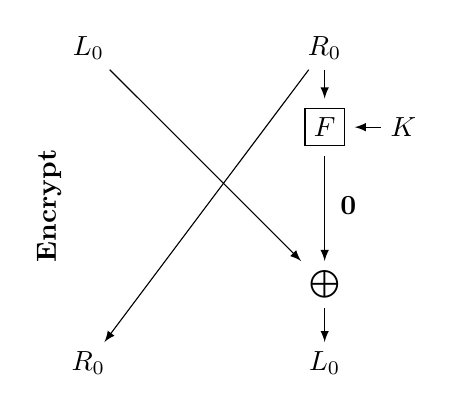
\begin{tikzpicture}

	% node definitions
	\node  (ip_left) at   (0,4) {$L_0$};
	\node (ip_right) at   (3,4) {$R_0$};
	\node      (des) at   (3,3) {$\boxed{F}$};
	\node      (key) at   (4,3) {$K$};
	\node     (zero) at (3.3,2) {$\mathbf{0}$};
	\node      (xor) at   (3,1) {$\bigoplus$};
	\node  (r1_left) at   (0,0) {$R_0$};
	\node (r1_right) at   (3,0) {$L_0$};

	% arrows
    \draw[-latex]  (ip_left) -- (xor);
    \draw[-latex] (ip_right) -- (r1_left);
	\draw[-latex] (ip_right) -- (des);
	\draw[-latex]      (key) -- (des);
	\draw[-latex]      (des) -- (xor);
	\draw[-latex]      (xor) -- (r1_right);

    % title
    \node[rotate=90] at (-0.5,2) {\textbf{Encrypt}};
	
\end{tikzpicture}
\end{document}